\documentclass[12pt,a4]{article}


\author{Yujie LU, Jiabao JI, Tong CHEN}
\newcommand{\handoutdate}{Friday, 2020-05-01}
\newcommand{\firstduedate}{Friday, 2020-05-08}
\newcommand{\finalduedate}{Tuesday, 2020-05-19}




\usepackage{graphicx,amsmath,amssymb,amsthm, boxedminipage}



\usepackage{algorithm}
\usepackage{algpseudocode}


\newtheorem{theorem}{Theorem}%[section]
\newtheorem{proposition}[theorem]{Proposition}
\newtheorem{lemma}[theorem]{Lemma}
\newtheorem{corollary}[theorem]{Corollary}
\newtheorem{definition}[theorem]{Definition}



\newcommand{\scalar}[2]{\ensuremath{\langle #1, #2\rangle}}
\newcommand{\floor}[1]{\left\lfloor #1 \right\rfloor}
\newcommand{\ceil}[1]{\left\lceil #1 \right\rceil}
\newcommand{\norm}[1]{\|#1\|}
\newcommand{\pfrac}[2]{\left(\frac{#1}{#2}\right)}
\newcommand{\nth}[1]{#1\textsuperscript{th}}

% \newcommand{\nth}[1]{#1\textsuperscript{th}}
\newcommand{\E}{\mathop{\mathbb{E\/}}}
\newcommand{\N}{\mathbb{N}}

\newcommand{\R}{\mathbb{R}}

\newtheorem{exercise}[theorem]{Exercise}
\newtheorem{exerciseD}[theorem]{*Exercise}
\newtheorem{exerciseDD}[theorem]{**Exercise}

\let\oldexercise\exercise
\renewcommand{\exercise}{\oldexercise\normalfont}

\let\oldexerciseD\exerciseD
\renewcommand{\exerciseD}{\oldexerciseD\normalfont}

\let\oldexerciseDD\exerciseDD
\renewcommand{\exerciseDD}{\oldexerciseDD\normalfont}


 
\begin{document}

\date{}

\title{CS 217 -- Algorithm Design and Analysis \\ 
  \vspace{3mm}
{\large	Shanghai Jiaotong University, Fall 2019\\
}
}
\maketitle

\noindent
Handed out on \handoutdate{}\\
First submission and questions due on \firstduedate{}\\
You will receive feedback from the TA.\\
Final submission due on \finalduedate{}




\setcounter{section}{4}
\section{More on Network Flows}

\begin{exercise}
    Let $G = (V,c)$ be a flow network. Prove that flow is ``transitive'' in the following sense: if $r,s,t$ are vertices, 
    and there is an $r$--$s$-flow of value $k$ and an $s$--$t$-flow of value $k$, then there is an $r$--$t$-flow of 
    value $k$.
\end{exercise}

\begin{proof}
	Denote the original r-s-flow and s-t-flow as $f_{rs}$ and $f_{st}$ respectively.
    We prove $f_{rt} = k$ by contradiction.

    Suppose $f_{rt} < k$, denote $f_{rt} = p$. By Max-Flow-Min-Cut THM, there is a cut $C$ 
    with $cap(C) = p < k$. If $s \in C$, we know that $C$ is also a r-s-cut. But by Max-Flow-Min-Cut
    THM, min $cap(r-s-cut) = k > cap(C) = p$, which leads to a contradiction. If $s \notin C$, the proof
    is similar. So $f_{rt} \ge k$, so there is a flow of value k in between $r, t$.
	
\end{proof}

\subsection{Vertex Disjoint Paths}

Let $G$ be a directed graph. Two paths $p_1, p_2$ from $s$ to $t$ are called {\em vertex disjoint}
if they don't share any vertices except $s$ and $t$. 

\begin{theorem}[Menger's Theorem]
   Let $G$ be a graph and $s \ne t$ two vertices therein. Let $k \in \mathbf{N}_0$. 
   Then exactly one of the following is true:
   \begin{enumerate}
   \item There are $k$ vertex disjoint paths $p_1,\dots,p_k$ from $s$ to $t$; that is, no two $p_i$, $p_j$ share
   any vertex besides $s$ and $t$.
   \item There are vertices $v_1,\dots,v_{k-1} \in V \setminus \{s,t\}$ such that
   $G - \{v_1,\dots, v_{k-1}\}$ contains no $s$--$t$-path.
   \end{enumerate}
\end{theorem}

\begin{exercise}
   Prove Menger's Theorem. You have to prove two things: first, not both cases above can occur (this is rather easy);
   second, one of them must occur (this requires a tool from the lecture).
\end{exercise}
\begin{proof}

	First we prove the easy part, these two cases will not occur simultaneously.Prove it by contradiction.

    Suppose both cases are true simultaneously, then there are $k$ vertex disjoint paths $p_1, ..., p_k$ from $s$ to $t$.
    and there exists $v_1, ..., v_{k - 1}$ such that $G - \{ v_1, ...,v_{k - 1}\}$ contains no 
    s-t-path. 
    
    For any $v_1, ..., v_{k - 1}$, the can take place in at most $k - 1$ paths in $p_1,...,p_k$ since $p_1, ..., p_k$ are
    disjoint vertex paths. Then we know there must be at least one path from $p_1,..,p_k$ left, which connects $s$ and $t$,
    leading to a contradiction.


    Next we prove that one of them must occur.

   For each vertex b, other than $s$ or $t$, replace b by the 2-vertex graph $H(b)$ with vertex set $\{b^+, b^−\}$ and arc $b^−b^+$ with cap $1$. Replace $s$ by $s^+$ and $t$ by $t^−$. Replace each edge $e=ab$, $\{a,b\}$  by the arcs $a^+b^−$ with cap $\inf$.
   
	If the maxinum flow of the new graph $G'$ is less than $k$. According to MaxFlow-MinCut Theroem and the min-cut must choose the edge $b^-b^+$, we can choose one of the min-cut that makes the graph has no s-t path and the number of points is less than $k$. That satisfies the situation 1.
	
	Otherwise, the maxinum flow is at least $k$, that means there are at least $k$ augmenting path in new graph $G'$. And we can correspond one augmenting path in new graph to one vertex disjoint paths in origin graph. That satisfies the situation 2.
\end{proof}


Let $V = \{0,1\}^n$. The $n$-dimensional Hamming cube $H_n$ is the graph $(V,E)$ where
$\{u,v\} \in E$ if $u,v$ differ in exactly one coordinate.
Define the $\nth{i}$ level of $H_n$ as 
\begin{align*}
  L_i := \{u \in V \ | \ \norm{u}_1 = i \} \ ,
\end{align*}
i.e., those vertices $u$ having exactly $i$ coordinates which are $1$.
\begin{center}
  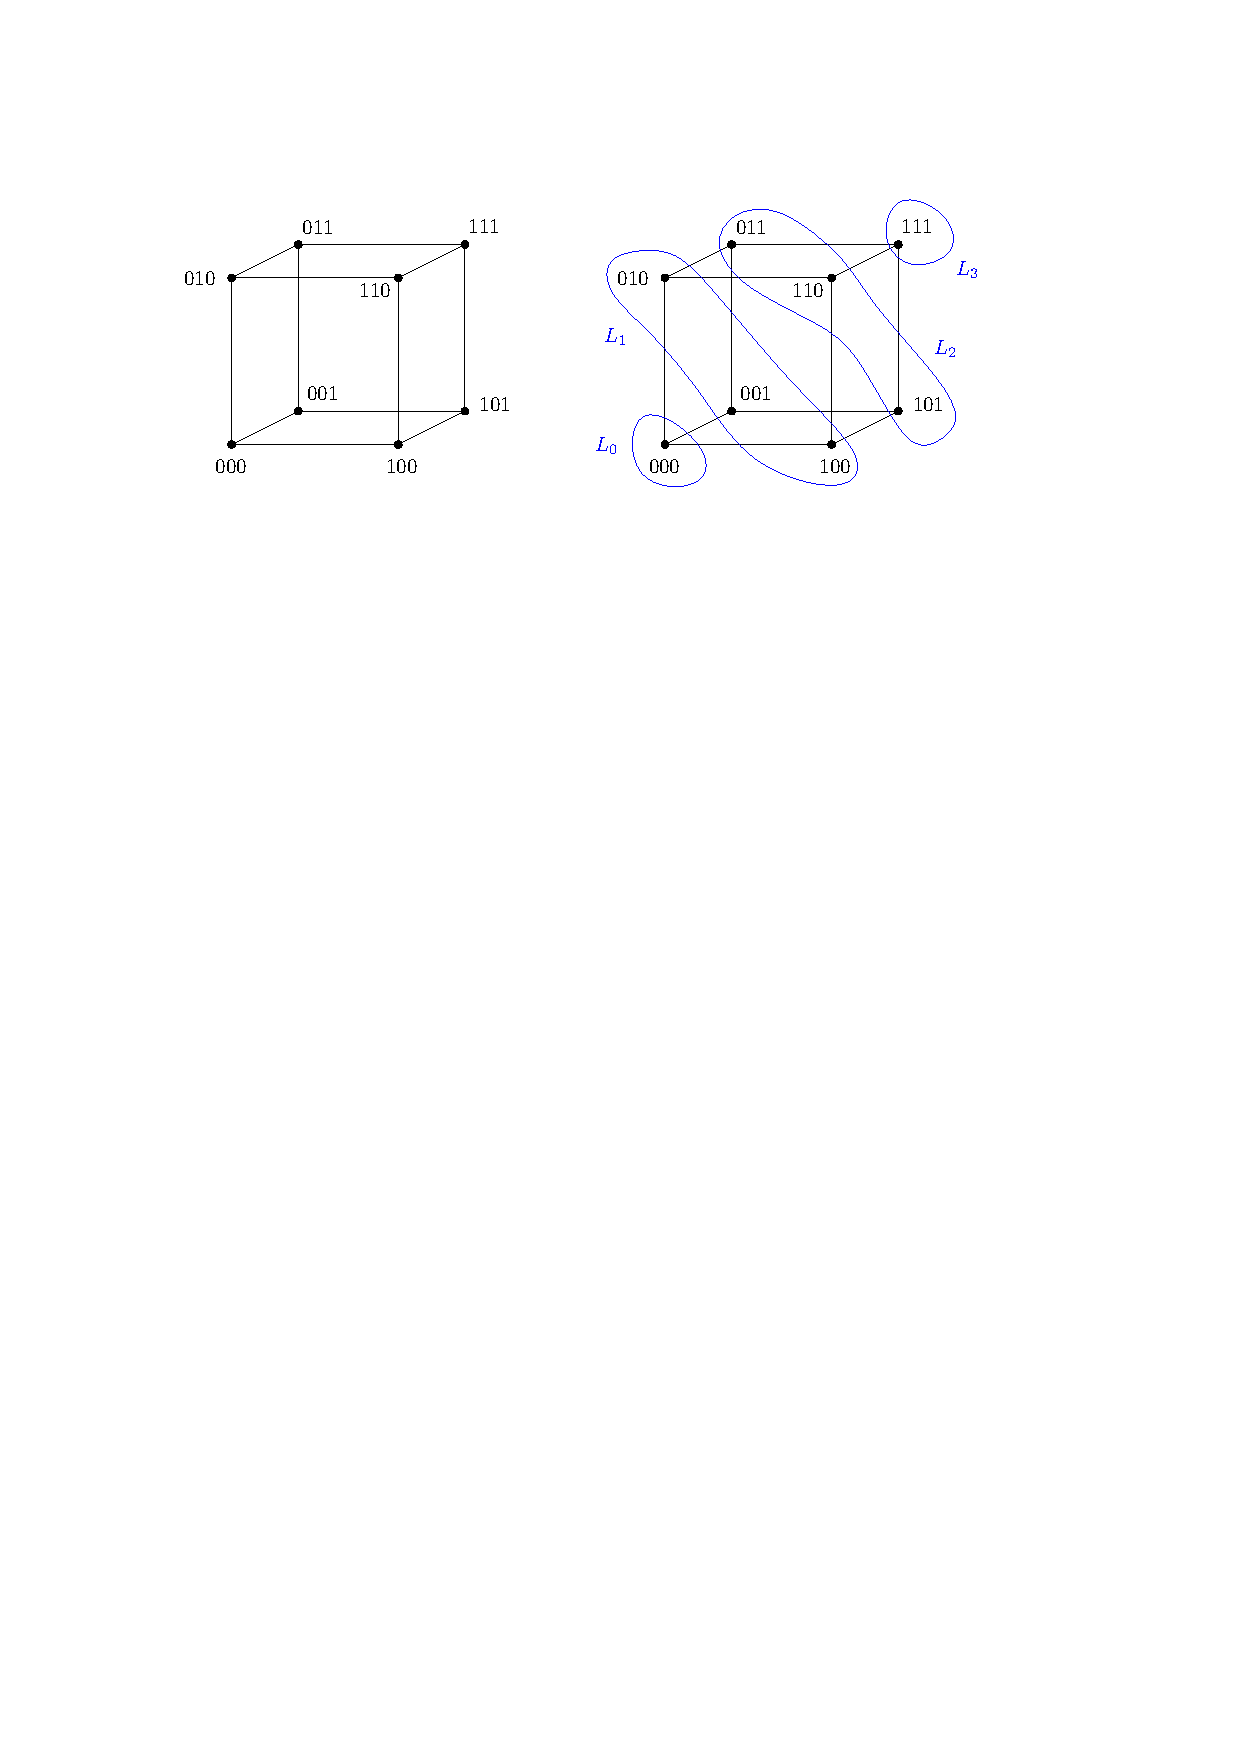
\includegraphics[width=0.8\textwidth]{figures/hamming-3-dim.pdf}\\
  {\small The $3$-dimensional Hamming cube and the four 
    sets $L_0$, $L_1$, $L_2$, $L_3$.}
\end{center}


\begin{exercise}[Matchings in $H_n$]
  Consider the induced bipartite subgraph $H_n[ L_i \cup L_{i+1}]$. This is 
  the graph on vertex set $L_i \cup L_{i+1}$ where two edges are connected
  by an edge if and only if they are connected in $H_n$.
  \medskip

  Show that for $i \leq n/2$ the graph $H_n[ L_i \cup L_{i+1}]$
  has a matching of size $|L_i| = {n \choose i}$.

\begin{center}
  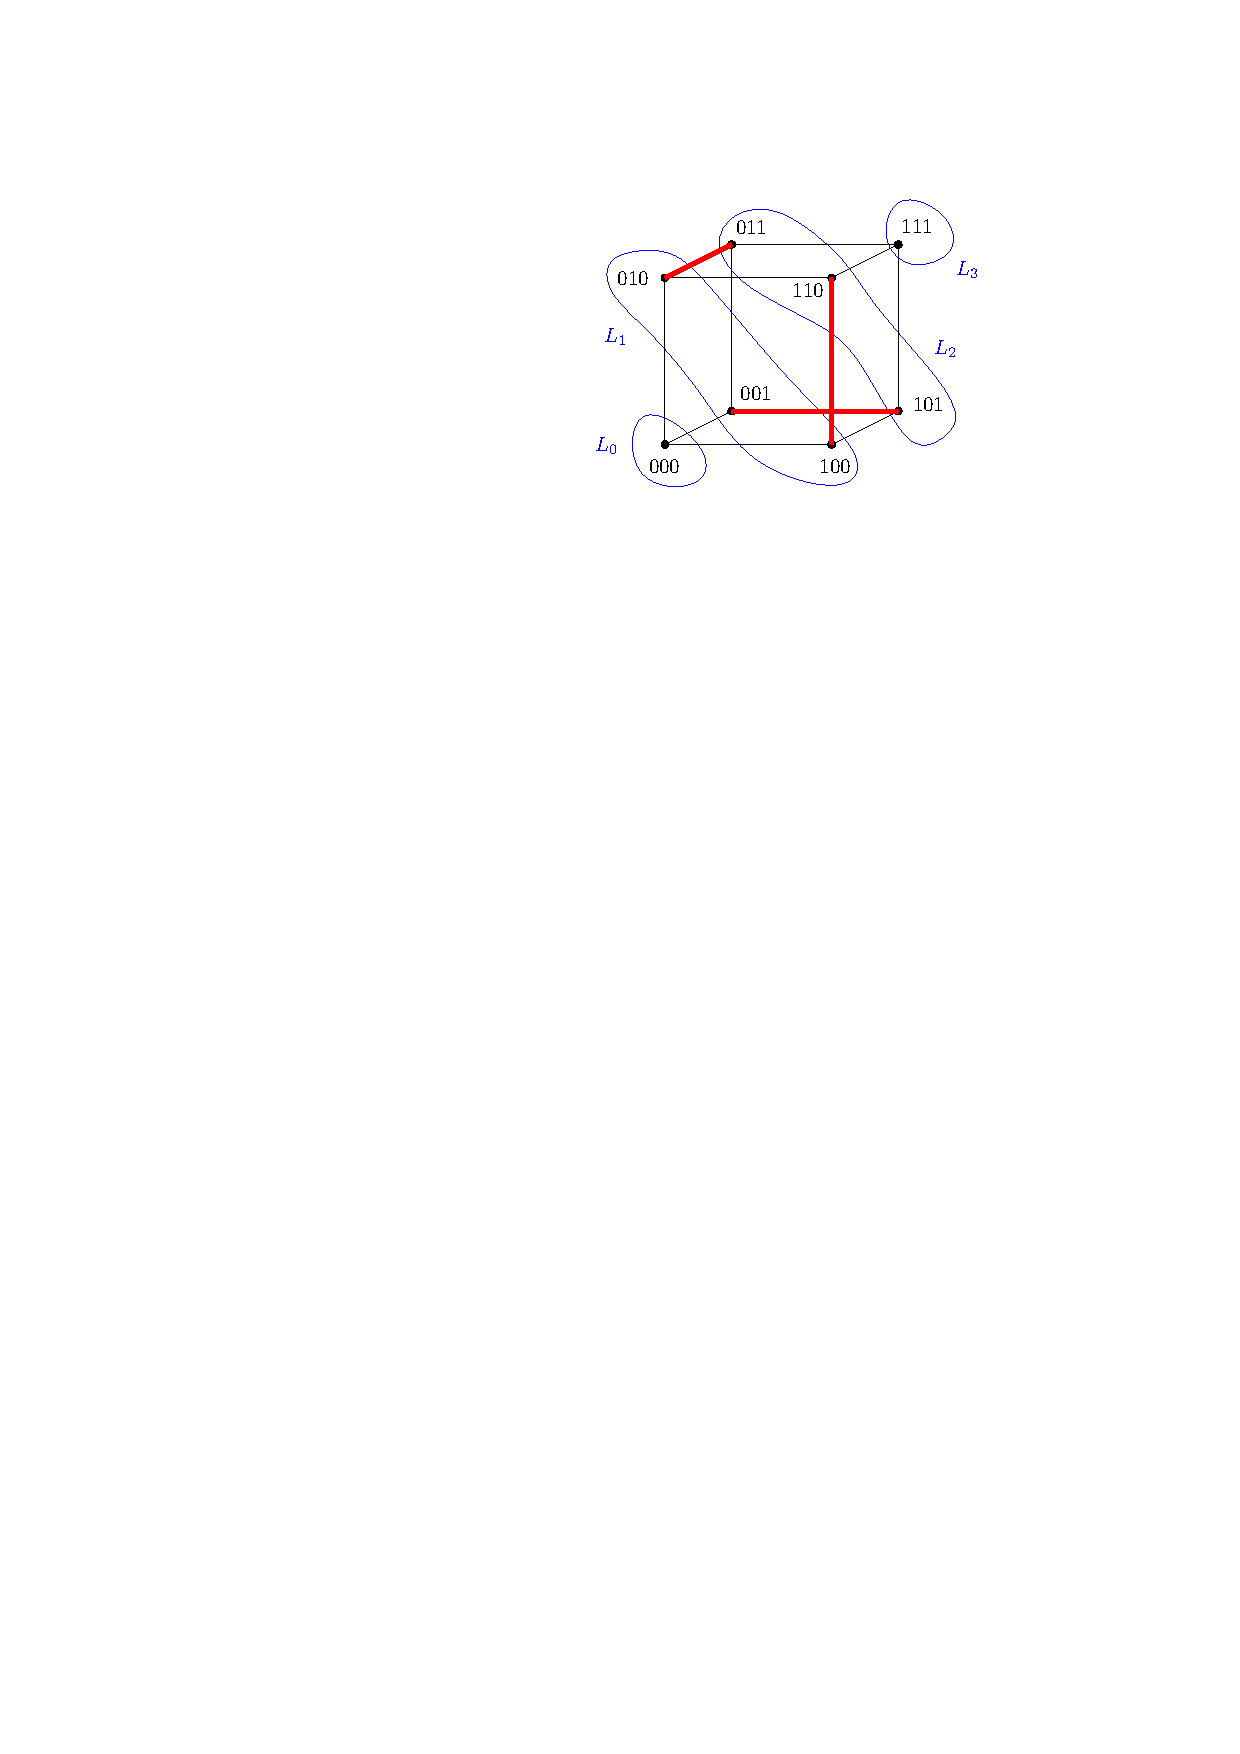
\includegraphics[width=0.4\textwidth]{figures/hamming-3-dim-matching.pdf}\\
  {\small A matching of size $3$ between $L_1$ and $L_2$.}
\end{center}
\label{exercise-matchings-in-H}
\end{exercise}
\begin{proof}
	On the left, sets of size $i$. On the right, sets of size $i + 1$, and an edge if the left vertex
is included in the right vertex. Note that every vertex on the left has $n-i$ neighbors, and every
vertex on the right has $i + 1$ neighbors.

	Let $S$ be any family of $L_i$. The number of edges coming out of S is $|S|(n-i)$, therefore,
the number of neighbors of S is at least $|S|(n-i)/(i+1) \ge |S|$. Hall’s theorem then completes
the proof.
\end{proof}
\begin{exercise} 
  Let $H_n$ be the $n$-dimensional Hamming cube. For $i < n/2$ consider
  $L_i$ and $L_{n-i}$. Note that 
  $|L_i| = {n \choose i} = { n \choose n-i}  = L_{n-i}$, so the 
  $L_i$ and $L_{n-i}$ have the same size.   Show that there are ${n \choose i}$ paths $p_1,p_2,\dots,p_{ {n \choose i}}$
  in $H_n$ such that
  (i) each $p_i$ starts in $L_i$ and ends in $L_{n-i}$;
  (ii) two different paths $p_i,p_j$ do not share any vertices.
  \textbf{Hint 1.} Model this problem as a network flow with vertex capacities. What would 
  the maximum flow be in this network?
  \textbf{Hint 2.} It's not {\em that} easy. If you try to work from both sides towards
  the middle by combining matchings between levels, 
  you will certainly run into problems as how to glue things together in the middle.
  I have never seen any ``meet in the middle'' proof that works.
  \textbf{Hint 3.} There is a ``direct'' proof by induction that does not require anything
  about network flows.

\end{exercise}
\begin{proof}

  We can build a new network like this, create a source vertex $s$ and a terminal vertex $t$.
  Connect $s$ with all nodes in $L_i$ and $v$ with all nodes in $L_{n - i}$, leave all edges between
  $L_i, L_{i + 1}$ as they were. Assign all edges with capacity 1. 
  
  The maximum flow in this network is no larger than $|L_i| = \tbinom{n}{i}$, since the number of edges connecting 
  to $s$ is $|L_i|$ and they all have capacity 1. Then we give a flow with value $|L_i|$, this should 
  tell us the maximum flow is $\tbinom{n}{i}$

  Here is an example.

  \begin{figure}[h]
    \centering
    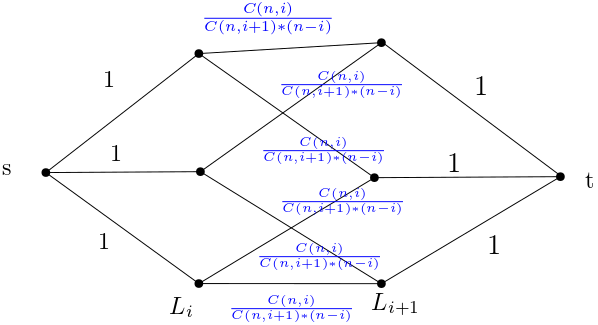
\includegraphics[scale=0.3]{figures/2.png}
    \caption{network}
  \end{figure}

  For all edges between $L_j, L_{j + 1}$, we assign it with flow 
  $\frac{C_{n}{i}}{C_{n}{j + 1} (n - j)}$ as the edges between $L_j,L_{j + 1}$ is 
  $C_{n}{j + 1}(n - j)$. Notice that $L_{j + 1}$ has $C_{n}{j + 1}$ nodes and each 
  node in $L_{j + 1}$ is connected with $(n - j)$ nodes in $L_j$.
  Since the graph is symmetrical, such flow can be built.

  Based on the proof of Menger's THM, we know that the maximum number of disjoint paths 
  equals the maximum flow in this network. So there're $\tbinom{n}{i}$
  disjoint paths from $L_i$ to $L_{n - i}$.

\end{proof}

\subsection{Matchings and Vertex Covers}

The following exercise was on the final exam of CS 499 (mathematical foundations of computer science) in spring 2019.
\begin{exercise}
    Let $\nu(G)$ denote the size of a maximum matching of $G$. Show that a bipartite graph $G$
    has at most $2^{\nu(G)}$ minimum vertex covers.
\end{exercise}
\begin{proof}

		Suppose the number of minimum vertex covers of graph $G$ is $m\left( G \right) $. We can easily 
\begin{figure}[ht]
    \centering
	\incfig[0.5]{example}
    \caption{example}
    \label{fig:example}
\end{figure}
Now we prove that there could be no more than $2^{\nu \left( G \right) }$ minimum vertex cover.
Let $G = A \cup B$, since $G$ is a bipartite graph. 
Assume that the maximum matching is $e_1,e_2,\ldots,e_t$, in which $t = \nu\left( G \right) $. By \textbf{Konig's Theorem} we know that the number of vertices in a minimum vertex cover is exactly $t$. 

Plus we can prove that every vertex in $K$, the vertex cover, is an endpoint of a matched edge. Hence the result is obvious.
\end{proof}
Obviously, this is not  true for general (non-bipartite) graphs: the triangle $K_3$ has $\nu(K_3) = 1$ but it has 
three minimum vertex covers. The five-cycle $C_5$ has $\nu(C_5) = 2$ but has five minimum vertex covers.

\begin{exercise}
   Is there a function $f: \mathbf{N}_0 \rightarrow \mathbf{N}_0$ such that every graph with $\nu(G) = k$ has 
   at most $f(k)$ minimum vertex covers? How small a function $f$ can you obtain?
\end{exercise}
\begin{proof}
	Assume that there are $m $ connected componets $G_1,\ldots,G_{m}$, and each have $c_{i} $ 
	vertexes, hence the number of minimum vertex 
cover is
\[
		S  = \prod_{i=1}^{m} c_{i} \le  f\left( k \right)  
.\] 
And suppose that connected component $G_{i}$ has maximum matching $k_{i}$.
We have $k_{i} \le  \frac{c_{i}}{2}$, therefore
\[
k = \sum_{i=1}^{m} k_i \le \frac{1}{2} \sum_{i=1}^{m} c_i
.\] 
Plus
\[
k = \sum_{i=1}^{m} k_i \ge m
.\] 
Hence we need to find the smallest function $f$ such that
 \[
		 \prod_{i=1}^{m} c_{i} \le   f\left( k \right) 
		 \le f\left( \frac{1}{2} \sum_{i=1}^{m} c_i \right) 
.\] 
Notice that 
\[
		\sum_{i=1}^{m} c_i \ge m \left( \prod_{i=1}^{m} c_i  \right) ^{\frac{1}{m}} 
.\] 
Let $t = \prod_{i=1}^{m} c_{i} $, we must have 
\[
		t\le f\left( \frac{m}{2} t ^{\frac{1}{m}} \right) 
.\] 
Which is equivalent to find the largest $g = f^{-1}$ such that
\[
	  \forall m, mt ^{\frac{1}{m} } -	2g\left( t \right)  \ge 0
.\] 
Thus $g$ cannot be polynomial, the maximum of $g$ could only be something like 
$c \ln\left( x \right) $ i.e.
\[
		h\left( t \right) = m t ^{\frac{1}{m}} - 2c\ln\left( t \right) , \forall t\ge 1,m\ge 1
.\] 
It easy to find the largest $c$ is  $\frac{1}{2}$. Hence the smallest $f$ is
$f\left( k \right) = e^{2k}$.

\end{proof}





\end{document}
